\section{Feature selection}\label{sec:featureselection}

A requirement for the Task 3.1 of the Project Specification is to select a
maximum of 10 ``good'' features to be used for the estimation of ECG's mean and
standard deviation. The initial list of features used is the one defined in the
\texttt{getfeatures} stage and described in \secref{subsec:getfeaturesstage}.

The script that performs the feature selection is \texttt{featureselection.m}.
It is divided in 2 parts: the first part extract the features using the
``Normal'' approach, while the second part does the same using the ``Windowed''
approach.

\subsection{Removing correlated features}\label{subsec:dropcorrelatedfeatures}

After features are extracted in the \texttt{extractfeatures} stage, they are
passed to the \texttt{findcorrelatedfeatures} stage which analyze the
correlation between features and divides the features in 2 list: correlated
(correlation coefficient \(\ge 0.8\)) and uncorrelated features. The
correlation matrix for the ``Normal'' case is shown
\vpageref{pdfinc:corrmatrix}. The correlation matrix for the ``Windowed'' case
is shown \vpageref{pdfinc:corrmatrixwindowed}. Those figures are quite big:
they can be zoomed since they are vectorial images. Anyway, for convenience,
\figref{fig:corrmatrixzoom} shows a zoom of the correlation matrices for both
cases.

\begin{figure}[!htb]
	\centering
	\begin{subfigure}{\textwidth}
		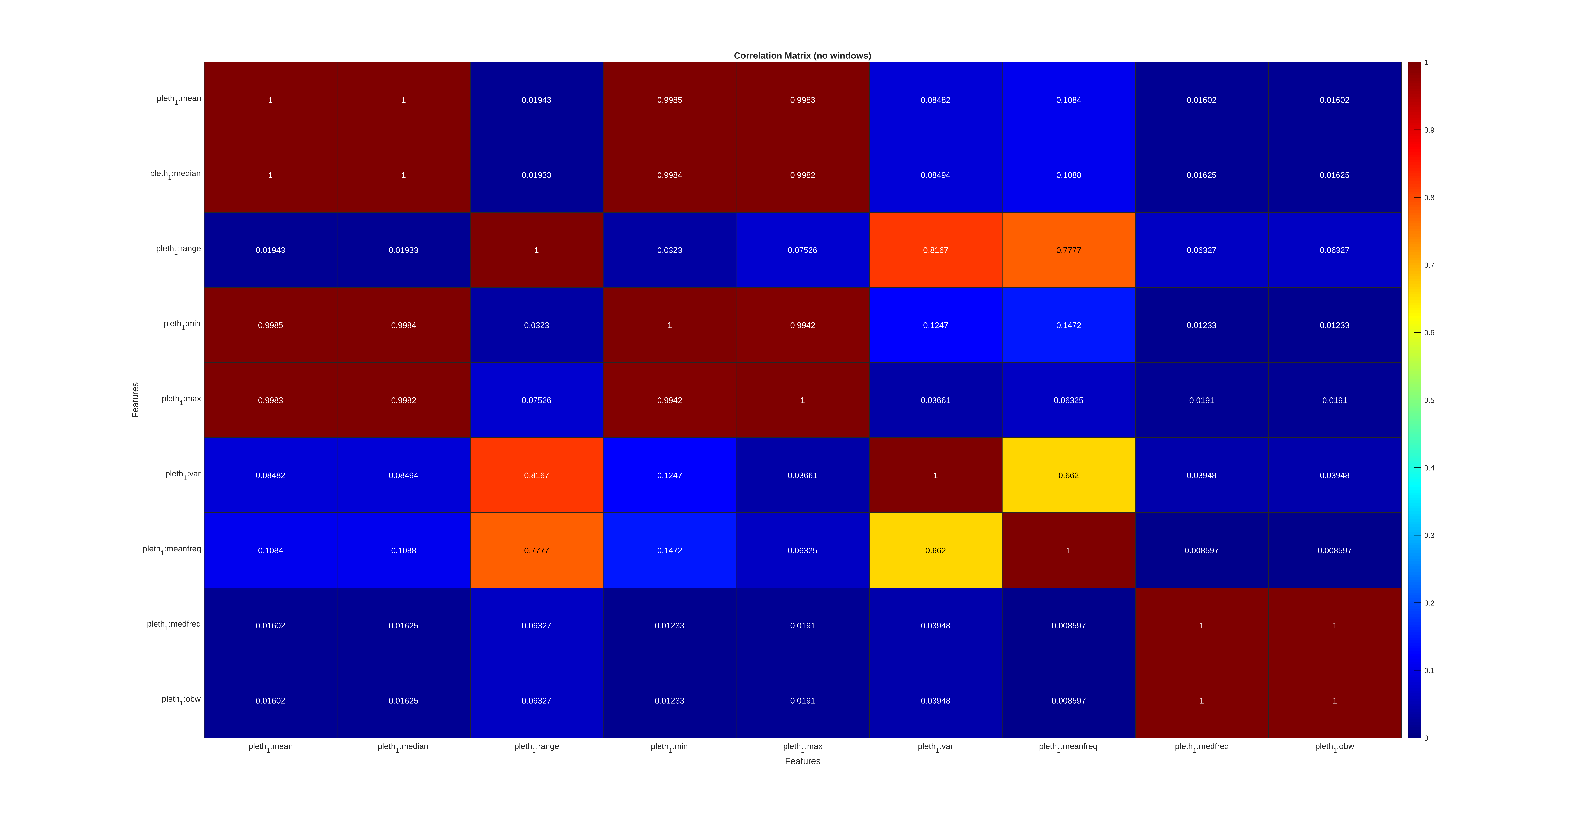
\includegraphics[width=\textwidth, trim=2.2cm 1.05cm 2.2cm 0.8cm, clip]{img/corrmatrixzoomnormal}
		\caption{``Normal'' case. The matrix shows, for example, the
		high correlation between the variance and the range for the
		\code{pleth\_1} signal.}\label{fig:corrmatrixzoomnormal}
	\end{subfigure}
	\begin{subfigure}{\textwidth}
		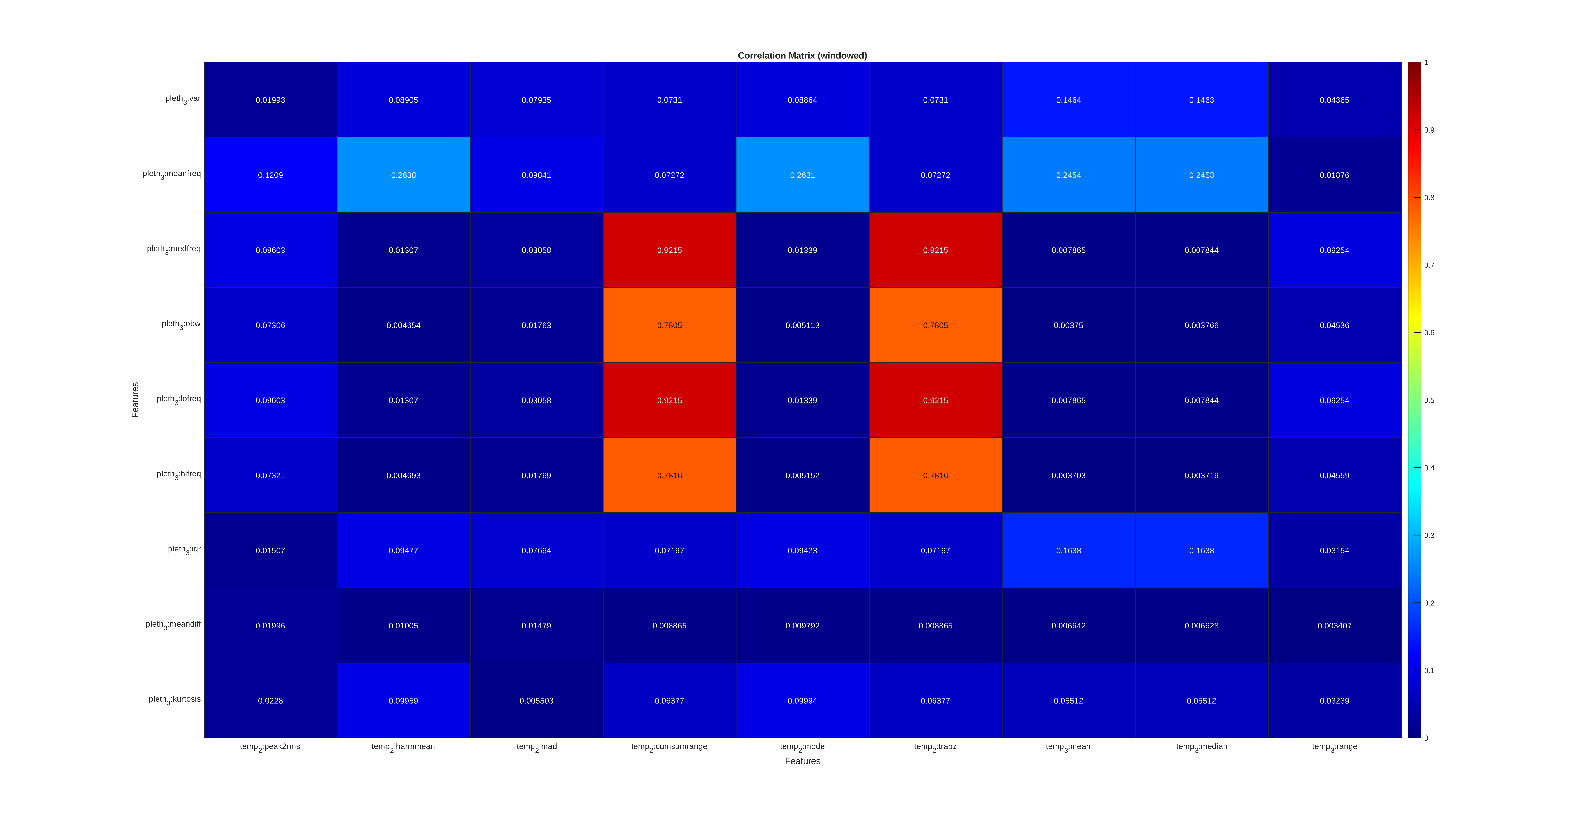
\includegraphics[width=\textwidth, trim=2.2cm 1.05cm 2.2cm 0.8cm, clip]{img/corrmatrixzoomwindowed}
		\caption{``Windowed'' case. The matrix shows, for example, the
		high correlation between the cumulative sum range and the
		trapezoidal integration of the \code{temp\_2} signal with some
		frequency domain features of the \code{pleth\_3}
		signal.}\label{fig:corrmatrixzoomwindowed}
	\end{subfigure}
	\caption{Zoom of the correlation matrices for the two feature
	extraction methods.}\label{fig:corrmatrixzoom}
\end{figure}

After that, the \texttt{dropcorrelatedfeatures} stage is called. This stage
removes the correlated features from the result of the \texttt{extractfeatures}
stage. 

\subsection{Selecting features with
\texttt{sequentialfs}}\label{subsec:sequentialfs}

The output of the \texttt{dropcorrelatedfeatures} stage is then normalized as
described in \secref{sec:normalization} and passed to the
\texttt{selectfeatures} stage which invokes the MATLAB's \code{sequentialfs}
function. Results of \code{sequentialfs}'s executions are shown in
\lstref{lst:sequentialfsnormal} and \lstref{lst:sequentialfswindowed}.

Note that, for the ``Windowed'' case, \code{sequentialfs} has been used to
select only 7 features instead of 10. This is because the test network used by
\code{sequentialfs} has a number of hidden neurons equal to \(\max
\{5,\lfloor\frac{N}{2}\rfloor\}\) where \(N\) is the number of input neurons
which is higher in the ``Windowed'' case (there is an input neuron for each
window for each feature), leading to a longer execution time for
\code{sequentialfs}.

\lstinputlisting[language={}, label={lst:sequentialfsnormal}, caption={Results
of \code{sequentialfs} execution for the ``Normal''
case.}]{sequentialfsnormal.txt}
\lstinputlisting[language={}, label={lst:sequentialfswindowed},
caption={Results of \code{sequentialfs} execution for the ``Windowed''
case.}]{sequentialfswindowed.txt}

For convenience, the list of selected features is also shown in
\tableref{table:selectedfeatures}.

\begin{table}[hbtp]
	\centering\footnotesize
	\begin{tabular}{r|c|c|c|c|}
		\toprule &
		\multicolumn{2}{|c|}{\standout{Normal}} &
		\multicolumn{2}{c|}{\standout{Windowed}} \\
		\hline &
		\standout{ECG mean} & \standout{ECG stddev} & \standout{ECG
		mean} & \standout{ECG stddev} \\
		\midrule
		1 & \code{pleth\_1:mean} & \code{lc\_1:mean} &
		\code{pleth\_1:mean} & \code{lc\_1:mean} \\
		2 & \code{lc\_1:mean} & \code{pleth\_2:mean} &
		\code{pleth\_2:mean} & \code{pleth\_2:mean} \\
		3 & \code{pleth\_3:mean} & \code{pleth\_3:mean} &
		\code{lc\_1:mean} & \code{temp\_1:mean} \\
		4 & \code{pleth\_4:mean} & \code{pleth\_1:mean} &
		\code{pleth\_3:mean} & \code{pleth\_1:mean} \\
		5 & \code{temp\_1:mean} & \code{temp\_1:mean} &
		\code{lc\_2:mean} & \code{pleth\_4:mean} \\
		6 & \code{pleth\_3:kurtosis} & \code{pleth\_4:meanfreq} &
		\code{pleth\_5:mean} & \code{lc\_2:mean} \\
		7 & \code{pleth\_6:meandiff} & \code{pleth\_1:meanfreq} &
		\code{lc\_2:meanfreq} & \code{pleth\_3:mean} \\
		8 & \code{temp\_3:var} & \code{lc\_2:mean} & & \\
		9 & \code{pleth\_5:skewness} & \code{pleth\_5:mean} & & \\
		10 & \code{pleth\_2:skewness} & \code{lc\_2:skewness} & & \\
		\bottomrule
	\end{tabular}
	\caption{List of features selected using MATLAB's
	\code{sequentialfs}.}\label{table:selectedfeatures}
\end{table}

\includepdf[pages={1}, landscape=true, fitpaper=true,
pagecommand={\thispagestyle{empty}\label{pdfinc:corrmatrix}}]{img/corrmatrix}

\includepdf[pages={1}, landscape=true, fitpaper=true,
pagecommand={\thispagestyle{empty}\label{pdfinc:corrmatrixwindowed}}]{img/corrmatrixwindowed}
